\documentclass[12pt,a4paper]{article}

% ─── Page Layout ───────────────────────────────────────────────────────────────
\usepackage[a4paper, margin=0.8in, headheight=14pt]{geometry}

% ─── Fonts (XeLaTeX) ───────────────────────────────────────────────────────────
\usepackage{fontspec}
\usepackage{unicode-math}
\setmainfont{TeX Gyre Pagella}
\setmonofont[Scale=0.88]{TeX Gyre Cursor}
\setmathfont{Latin Modern Math}

% ─── Packages ──────────────────────────────────────────────────────────────────
\usepackage{xcolor}
\usepackage{colortbl}
\usepackage{titlesec}
\usepackage{enumitem}
\usepackage{tabularx}
\usepackage{booktabs}
\usepackage{array}
\usepackage{amsmath}
\usepackage{tikz}
\usetikzlibrary{shapes.geometric, arrows.meta, positioning, calc, fit, decorations.pathreplacing}
\usepackage{tcolorbox}
\tcbuselibrary{skins, breakable}
\usepackage{hyperref}
\usepackage{fancyhdr}
\usepackage{graphicx}
\usepackage{microtype}
\hyphenpenalty=10000
\exhyphenpenalty=10000
\sloppy
\usepackage{caption}
\usepackage{setspace}
\usepackage{multirow}
\usepackage{tocloft}

% ─── Q&A helper ────────────────────────────────────────────────────────────────
\newcommand{\Q}[1]{\textbf{#1}\par\noindent\ignorespaces}

% ─── Colour Palette ────────────────────────────────────────────────────────────
\definecolor{myred}{RGB}{196,30,58}
\definecolor{mydark}{RGB}{30,30,50}
\definecolor{mygreen}{RGB}{14,120,80}
\definecolor{myteal}{RGB}{0,130,140}
\definecolor{myamber}{RGB}{180,100,0}
\definecolor{mypurple}{RGB}{100,30,160}
\definecolor{mygray}{RGB}{246,247,249}
\definecolor{mgframe}{RGB}{180,185,200}
\definecolor{watermark}{RGB}{145,150,170}
\definecolor{hdrred}{RGB}{250,232,235}
\definecolor{hdrgreen}{RGB}{220,244,233}
\definecolor{hdrteal}{RGB}{220,242,244}
\definecolor{hdramber}{RGB}{253,242,215}
\definecolor{hdrpurple}{RGB}{238,228,255}
\definecolor{hdrgray}{RGB}{238,240,245}
\definecolor{rowalt}{RGB}{250,251,253}

% ─── Section Formatting ────────────────────────────────────────────────────────
\titleformat{\section}
  {\large\bfseries\color{myred}}{\thesection.}{0.5em}{}
  [\vspace{1pt}{\color{myred}\rule{\linewidth}{0.8pt}}]
\titleformat{\subsection}
  {\normalsize\bfseries\color{myteal}}{\thesubsection}{0.5em}{}
\titlespacing*{\section}{0pt}{18pt}{7pt}
\titlespacing*{\subsection}{0pt}{11pt}{4pt}

% ─── Paragraph ─────────────────────────────────────────────────────────────────
\setlength{\parindent}{0pt}
\setlength{\parskip}{4pt}

% ─── TOC Styling ───────────────────────────────────────────────────────────────
\renewcommand{\cfttoctitlefont}{\large\bfseries\color{myred}}
\renewcommand{\cftaftertoctitle}{\par\noindent{\color{myred}\rule{\linewidth}{0.8pt}}}
\setlength{\cftbeforetoctitleskip}{0pt}
\setlength{\cftaftertoctitleskip}{6pt}
\renewcommand{\cftsecfont}{\normalsize\bfseries\color{mydark}}
\renewcommand{\cftsecpagefont}{\normalsize\bfseries\color{mydark}}
\renewcommand{\cftsecleader}{\cftdotfill{\cftdotsep}}
\setlength{\cftbeforesecskip}{7pt}
\renewcommand{\cftsubsecfont}{\small\color{mydark}}
\renewcommand{\cftsubsecpagefont}{\small\color{mydark}}
\setlength{\cftbeforesubsecskip}{3pt}
\setlength{\cftsubsecindent}{1.4em}

% ─── Table helpers ─────────────────────────────────────────────────────────────
\renewcommand{\arraystretch}{1.45}
\setlength{\tabcolsep}{6pt}
\arrayrulecolor{mydark}
\newcolumntype{B}[1]{>{\small\bfseries\raggedright\arraybackslash}m{#1}}
\newcolumntype{Y}{>{\small\raggedright\arraybackslash}X}
\renewcommand{\tabularxcolumn}[1]{m{#1}}

% ─── Header / Footer ───────────────────────────────────────────────────────────
\pagestyle{fancy}
\fancyhf{}
\fancyhead[L]{\small\color{myred}\textbf{PE-EC702C}\;\color{mydark}--- Neural Network and Fuzzy Logic Control}
\fancyhead[R]{\small\color{myteal}\textbf{Module 5 Notes}}
\fancyfoot[C]{\small\color{mydark}\thepage}
\fancyfoot[R]{\small\color{watermark}\textit{\copyright\ Biraj}}
\renewcommand{\headrulewidth}{0.5pt}
\renewcommand{\footrulewidth}{0.3pt}

% ─── Hyperref ──────────────────────────────────────────────────────────────────
\hypersetup{
  colorlinks=true, linkcolor=myteal, urlcolor=myteal,
  pdfauthor={Biraj Sarkar},
  pdftitle={PE-EC702C --- Module 5 Notes}
}

% ─── tcolorbox styles ──────────────────────────────────────────────────────────
\tcbset{
  tikzbox/.style={
    colback=mygray, colframe=mgframe, boxrule=0.6pt, arc=4pt,
    left=8pt, right=8pt, top=6pt, bottom=6pt,
    colbacktitle=mgframe, coltitle=mydark,
    fonttitle=\small\bfseries
  },
  defbox/.style={
    colback=hdrgreen, colframe=mygreen, boxrule=0.8pt, arc=4pt,
    left=9pt, right=9pt, top=6pt, bottom=6pt,
    colbacktitle=mygreen, coltitle=white,
    fonttitle=\small\bfseries
  },
  formulabox/.style={
    colback=hdrteal, colframe=myteal, boxrule=0.8pt, arc=4pt,
    left=9pt, right=9pt, top=7pt, bottom=7pt,
    colbacktitle=myteal, coltitle=white,
    fonttitle=\small\bfseries
  },
  examplebox/.style={
    colback=hdramber, colframe=myamber, boxrule=0.8pt, arc=4pt,
    left=9pt, right=9pt, top=6pt, bottom=6pt,
    colbacktitle=myamber, coltitle=white,
    fonttitle=\small\bfseries,
    breakable
  },
  masonbox/.style={
    colback=hdrpurple, colframe=mypurple, boxrule=0.8pt, arc=4pt,
    left=9pt, right=9pt, top=6pt, bottom=6pt,
    colbacktitle=mypurple, coltitle=white,
    fonttitle=\small\bfseries
  },
  exambox/.style={
    colback=hdrpurple, colframe=mypurple, boxrule=1pt, arc=5pt,
    left=10pt, right=10pt, top=8pt, bottom=8pt,
    colbacktitle=mypurple, coltitle=white,
    fonttitle=\bfseries,
    breakable, title after break={\textbf{Frequently Asked / Viva Questions (contd.)}}}
}
\tcbset{breakable}

% ─── TikZ styles ───────────────────────────────────────────────────────────────
\tikzset{
  block/.style={rectangle, draw=myteal, fill=hdrteal,
    text width=2.2cm, align=center, minimum height=0.85cm,
    font=\small, rounded corners=3pt, line width=0.7pt},
  arrow/.style={-Stealth, thick, color=mydark},
  line/.style={thick, color=mydark}
}

% ═══════════════════════════════════════════════════════════════════════════════
\begin{document}
% ═══════════════════════════════════════════════════════════════════════════════

\begin{center}
  {\LARGE\bfseries\color{myred} PE-EC702C --- Neural Network \& Fuzzy Logic Control}\\[5pt]
  {\normalsize\color{mydark} Semester VII \quad$\bullet$\quad 3L:0T:0P \quad$\bullet$\quad 3 Credits}\\[3pt]
  {\normalsize\color{myteal}\textbf{Module 5 Exam Notes: Applications of Neural Networks \& Fuzzy Logic}}\\[3pt]
  {\small\color{mydark} CGEC \;$|$\; B.Tech ECE (2023--27) \;$|$\; \textit{Biraj Sarkar}}
\end{center}
\vspace{2pt}
\noindent{\color{myred}\rule{\linewidth}{1.5pt}}
\vspace{2pt}

\hypersetup{linkcolor=mydark}
\tableofcontents
\hypersetup{linkcolor=myteal}
\newpage

% ===============================================================================
\section{Applications of Artificial Neural Networks}
% ===============================================================================

Neural networks excel at pattern recognition, function approximation, and adaptive modeling due to their parallel distributed architecture and learning capabilities.

\begin{enumerate}[leftmargin=*, itemsep=4pt]
  \item \textbf{Pattern and Character Recognition:} ANNs (particularly CNNs and MLPs) are widely used for Optical Character Recognition (OCR), signature verification, and face recognition by learning translation-invariant spatial features.
  \item \textbf{Image Compression:} Feedforward networks with a narrow hidden layer (bottleneck autoencoders) perform dimensionality reduction. The input image is reconstructed at the output layer, while the compressed representation is stored at the hidden layer.
  \item \textbf{Communication Systems (Channel Equalization):} Equalizers modeled using neural networks (like radial basis function networks) reduce Inter-Symbol Interference (ISI) in dispersive channels by acting as non-linear classifiers.
  \item \textbf{Control Systems (System Identification):} ANNs model the forward and inverse dynamics of complex, non-linear chemical and mechanical processes, facilitating adaptive and predictive control schemes.
\end{enumerate}

% ===============================================================================
\section{Applications of Fuzzy Logic}
% ===============================================================================

Fuzzy logic is highly effective in systems involving linguistic variables and human decision-making processes, where exact mathematical models are unavailable.

\begin{itemize}[leftmargin=*, itemsep=3pt]
  \item \textbf{Fuzzy Pattern Recognition:} Classifies inputs into overlapping classes based on membership values rather than crisp thresholds.
  \item \textbf{Fuzzy Image Compression:} Uses fuzzy rules to adaptively select quantization levels across different image blocks based on local edge/texture complexity.
\end{itemize}

% ===============================================================================
\section{Fuzzy Logic Controllers (FLC)}
% ===============================================================================

A Fuzzy Logic Controller (FLC) implements a control algorithm by evaluating heuristic, rule-based statements rather than mathematical differential equations.

\begin{tcolorbox}[tikzbox, title={Fuzzy Logic Controller Block Diagram}]
\centering
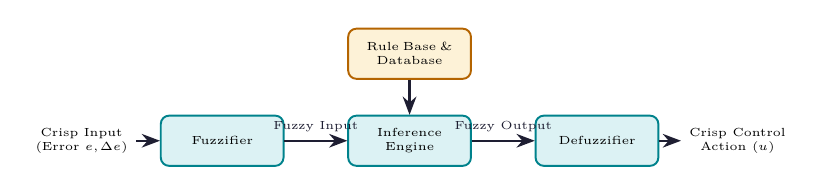
\begin{tikzpicture}[scale=0.85, every node/.style={transform shape, font=\tiny},
  block/.style={rectangle, draw=myteal, fill=hdrteal,
    text width=1.6cm, align=center, minimum height=0.75cm,
    font=\tiny, rounded corners=3pt, line width=0.7pt}]
  
  % Blocks
  \node[block] (fuzz) at (0, 0) {Fuzzifier};
  \node[block] (infer) at (2.8, 0) {Inference\\Engine};
  \node[block] (defuzz) at (5.6, 0) {Defuzzifier};
  
  \node[block, draw=myamber, fill=hdramber] (rules) at (2.8, 1.3) {Rule Base \&\\Database};

  % Inputs & Outputs
  \node (in) at (-2.1, 0) [align=center, font=\fontsize{5}{6}\selectfont] {Crisp Input\\(Error $e, \Delta e$)};
  \node (out) at (7.7, 0) [align=center, font=\fontsize{5}{6}\selectfont] {Crisp Control\\Action ($u$)};

  % Connections
  \draw[arrow] (in) -- (fuzz);
  \draw[arrow] (fuzz) -- node[midway, above, font=\fontsize{5}{6}\selectfont\color{myteal}] {Fuzzy Input} (infer);
  \draw[arrow] (infer) -- node[midway, above, font=\fontsize{5}{6}\selectfont\color{myteal}] {Fuzzy Output} (defuzz);
  \draw[arrow] (defuzz) -- (out);
  
  \draw[arrow] (rules.south) -- (infer.north);
\end{tikzpicture}
\end{tcolorbox}

\subsection{Standard FLC Architecture Components}
\begin{enumerate}[leftmargin=*, itemsep=3.5pt]
  \item \textbf{Fuzzifier (Fuzzification Interface):} Measures physical inputs and converts them into fuzzy values (linguistic terms like *Positive Big*, *Zero*, *Negative Small*) using predefined input membership functions.
  \item \textbf{Knowledge Base (Rule \& Database):} Contains the database (definitions of membership functions) and the Rule Base (a collection of linguistic control statements in \textbf{IF-THEN} format).
  \item \textbf{Inference Engine (Decision Making Logic):} Evaluates the active rules to determine the overall fuzzy control output based on composition rules (usually Max-Min composition).
  \item \textbf{Defuzzifier (Defuzzification Interface):} Converts the combined fuzzy output into a single crisp control command to drive physical actuators.
\end{enumerate}

% ===============================================================================
\section{Control System Case Studies}
% ===============================================================================

\subsection{Inverted Pendulum Controller}
The goal is to maintain a rotating pole in an upright position by moving a motorized cart horizontally.

\begin{tcolorbox}[tikzbox, title={Inverted Pendulum Physical Model}]
\centering
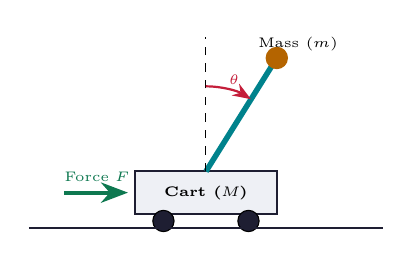
\begin{tikzpicture}[scale=0.9, every node/.style={font=\tiny}]
  % Cart
  \draw[thick, fill=hdrgray, draw=mydark] (-1, 0) rectangle (1, 0.6);
  \draw[fill=mydark] (-0.6, -0.1) circle (0.15);
  \draw[fill=mydark] (0.6, -0.1) circle (0.15);
  \node at (0, 0.3) {\textbf{Cart ($M$)}};

  % Ground
  \draw[line] (-2.5, -0.2) -- (2.5, -0.2);

  % Pendulum Pole
  \draw[line, line width=2pt, color=myteal] (0, 0.6) -- (1.0, 2.2);
  \draw[fill=myamber, draw=myamber] (1.0, 2.2) circle (0.15);
  \node at (1.3, 2.4) {Mass ($m$)};
  
  % Angle
  \draw[dashed] (0, 0.6) -- (0, 2.5);
  \draw[arrow, color=myred] (0, 1.8) arc (90:58:1.2);
  \node at (0.4, 1.9) [color=myred] {$\theta$};

  % Force arrow
  \draw[arrow, line width=1.5pt, color=mygreen] (-2.0, 0.3) -- (-1.1, 0.3) node[midway, above] {Force $F$};
\end{tikzpicture}
\end{tcolorbox}

\par\noindent
\begin{itemize}[leftmargin=*, itemsep=3pt]
  \item \textbf{Inputs:} Angle error $\theta$ (deviation from vertical) and angular velocity $e_{\omega} = d\theta/dt$.
  \item \textbf{Output:} Motor force $F$ applied to the cart.
  \item \textbf{Rule Base example:}
    \begin{itemize}[leftmargin=1.5em]
      \item \textit{IF angle ($\theta$) is Positive Small AND angular velocity ($d\theta/dt$) is Zero, THEN force ($F$) is Positive Small.}
    \end{itemize}
\end{itemize}

\subsection{Fuzzy Washing Machine Controller}
An FLC optimizes the wash cycle time, water temperature, and spin speed based on:
\begin{itemize}[leftmargin=*, itemsep=3pt]
  \item \textbf{Inputs:} Dirtiness level of clothes (using optical sensors that measure water transparency) and weight of load.
  \item \textbf{Output:} Cycle duration (wash time).
  \item \textbf{Rule Base example:}
    \begin{itemize}[leftmargin=1.5em]
      \item \textit{IF dirtiness is High AND weight is Medium, THEN wash time is Long.}
    \end{itemize}
\end{itemize}

% ===============================================================================
\section{Worked Examples}
% ===============================================================================

\begin{tcolorbox}[examplebox, title={Fuzzy Inference System Evaluation}]
\textbf{Problem:} Consider a simple Fuzzy Logic Controller with two input variables $x$ (error) and $y$ (change of error), and one output $z$ (control force).
The fuzzy rule base contains the following two rules:
\begin{itemize}[leftmargin=*, itemsep=2pt]
  \item \textbf{Rule 1:} IF $x$ is $A_1$ AND $y$ is $B_1$, THEN $z$ is $C_1$
  \item \textbf{Rule 2:} IF $x$ is $A_2$ AND $y$ is $B_2$, THEN $z$ is $C_2$
\end{itemize}

Given crisp input values $x_0 = 4$ and $y_0 = 6$:
\begin{itemize}[leftmargin=*, itemsep=2pt]
  \item Membership values: $\mu_{A_1}(x_0) = 0.6, \quad \mu_{A_2}(x_0) = 0.3, \quad \mu_{B_1}(y_0) = 0.8, \quad \mu_{B_2}(y_0) = 0.4$
  \item Output membership centers (represented by singletons): $z_{C_1} = 20, \quad z_{C_2} = 50$
\end{itemize}
Evaluate the output control value $z^*$ using the \textbf{weighted average} defuzzification method.
\par\vspace{4pt}\noindent\rule{\linewidth}{0.5pt}\par
\textbf{Solution:}

\textbf{1. Compute Firing Strengths ($\alpha$-levels) of the rules:}
Since the connective is \textbf{AND}, we use the Min operator:
\begin{itemize}[leftmargin=*, itemsep=2.5pt]
  \item For \textbf{Rule 1}:
    \begin{equation*}
      \alpha_1 = \min\left( \mu_{A_1}(x_0), \mu_{B_1}(y_0) \right) = \min(0.6, 0.8) = 0.6
    \end{equation*}
  \item For \textbf{Rule 2}:
    \begin{equation*}
      \alpha_2 = \min\left( \mu_{A_2}(x_0), \mu_{B_2}(y_0) \right) = \min(0.3, 0.4) = 0.3
    \end{equation*}
\end{itemize}

\par\vspace{4pt}
\textbf{2. Calculate Defuzzified Output ($z^*$):}
Using the weighted average formula:
\begin{align*}
  z^* &= \frac{\alpha_1 z_{C_1} + \alpha_2 z_{C_2}}{\alpha_1 + \alpha_2} \\
  &= \frac{0.6(20) + 0.3(50)}{0.6 + 0.3} \\
  &= \frac{12 + 15}{0.9} = \frac{27}{0.9} = 30
\end{align*}
The output control force is $z^* = 30$.
\end{tcolorbox}

\newpage

% ===============================================================================
% MANDATORY QUICK REVISION PAGE
% ===============================================================================
\begin{center}
  {\large\bfseries\color{myred} Quick Revision --- Module V}\\[3pt]
  {\small\color{mydark} Applications of Neural Networks \& Fuzzy Logic $|$ PE-EC702C}
\end{center}
\noindent{\color{myred}\rule{\linewidth}{1.2pt}}
\vspace{4pt}

\begin{tcolorbox}[formulabox, title={\textbf{Key Formulas at a Glance}}]
\renewcommand{\arraystretch}{1.3}
\begin{tabularx}{\linewidth}{B{5.0cm} X}Rule Firing Strength (AND) & $\alpha_i = \min\left( \mu_{A_i}(x_0), \mu_{B_i}(y_0) \right)$ \\
Rule Firing Strength (OR) & $\alpha_i = \max\left( \mu_{A_i}(x_0), \mu_{B_i}(y_0) \right)$ \\
Weighted Average Defuzzification & $z^* = \frac{\sum \alpha_i z_i}{\sum \alpha_i}$ \\
Inverted Pendulum Angle Error & $e(t) = \theta_{ref} - \theta(t)$ \\
Inverted Pendulum Error Change & $\Delta e(t) = e(t) - e(t-1)$
\end{tabularx}
\tcbset{colbacktitle=myteal, coltitle=white}
\end{tcolorbox}

\begin{tcolorbox}[defbox, title={\textbf{One-Line Definitions}}]
\begin{itemize}[leftmargin=*, itemsep=2.5pt, topsep=0pt]
  \item \textbf{Fuzzy Controller:} A control device that uses linguistic rules and fuzzy reasoning to calculate system control inputs.
  \item \textbf{Fuzzifier:} The interface in an FLC that maps physical crisp sensor readings to linguistic fuzzy values.
  \item \textbf{Inference Engine:} The decision-making unit that evaluates active rule statements to determine control signals.
  \item \textbf{Linguistic Variable:} A variable whose values are words or sentences in a language rather than numbers (e.g. "Warm").
  \item \textbf{System Identification:} The process of developing a mathematical or neural network model to describe dynamic process behavior.
\end{itemize}
\tcbset{colbacktitle=myteal, coltitle=white}
\end{tcolorbox}

\begin{tcolorbox}[exambox, title={\textbf{Frequently Asked / Viva Questions}}]
\begin{enumerate}[leftmargin=*, itemsep=3.5pt, label=\arabic*.]
  \item \Q{What are the main advantages of a Fuzzy Logic Controller over a PID controller?} FLCs do not require an exact mathematical model of the process, can handle non-linear dynamics easily, and can incorporate human operator heuristics directly using linguistic rules.
  \item \Q{State the function of the FLC Rule Base.} The Rule Base contains the control logic written as a set of IF-THEN rules that describe the relationship between input error conditions and output control actions.
  \item \Q{How is a neural network used for image compression?} An autoencoder network is trained to replicate inputs at its output layer. A bottleneck hidden layer (fewer nodes) forces the network to learn a compressed representation of the image.
  \item \Q{What is channel equalization in communications, and how do ANNs help?} Channel equalization compensates for signal distortion (ISI) caused by transmission channels. ANNs act as adaptive classifiers that identify non-linear decision boundaries to recover transmitted symbols.
  \item \Q{Explain the wash time optimization in a fuzzy washing machine.} Sensors measure the quantity of load and the dirtiness of the water (transparency). The FLC infers the optimum wash cycle time: muddy water with a heavy load triggers a long wash cycle.
  \item \Q{What inputs are required to balance an inverted pendulum?} The deviation angle $\theta$ from the vertical axis (error) and the rate of change of the angle $d\theta/dt$ (angular velocity).
  \item \Q{What is the difference between Mamdani and Sugeno fuzzy inference systems?} Mamdani systems use fuzzy sets for output membership functions, requiring defuzzification. Sugeno systems use linear mathematical functions or constants for outputs, simplifying calculation.
  \item \Q{Define a Singleton membership function.} A singleton is a membership function that has a value of $1.0$ at a single specific point and $0$ everywhere else.
  \item \Q{How does a neural network model non-linear control systems?} By acting as a system identification model, learning the mapping between system input history and corresponding output responses.
  \item \Q{What is the role of the database in a fuzzy controller?} The database holds the exact parameters (shapes, coordinates, limits) of the membership functions defined for the input and output variables.
\end{enumerate}
\tcbset{colbacktitle=myteal, coltitle=white}
\end{tcolorbox}

\begin{tcolorbox}[tikzbox, title={Comparison of Control Strategies}]
\centering
{\renewcommand{\arraystretch}{1.55}%
\begin{tabularx}{\linewidth}{|>{\bfseries}B{3.2cm}|Y|Y|}
\hline
Parameter & Classical PID Control & Fuzzy Logic Control \\
\hline
Process Model & Requires exact mathematical model & No mathematical model required \\
\hline
Control Logic & Defined by differential equations & Defined by linguistic IF-THEN rules \\
\hline
Tuning Parameters & Proportional, Integral, Derivative gains & Membership functions and rule parameters \\[4pt]
\hline
Non-linear Handling & Difficult (often requires linearization) & Inherently handles non-linearities \\[4pt]
\hline
\end{tabularx}}
\tcbset{colbacktitle=myteal, coltitle=white}
\end{tcolorbox}

\end{document}
